% SPDX-License-Identifier: CC-BY-SA-4.0
%
% Copyright (c) 2020 Philipp Le
%
% Except where otherwise noted, this work is licensed under a
% Creative Commons Attribution-ShareAlike 4.0 License.
%
% Please find the full copy of the licence at:
% https://creativecommons.org/licenses/by-sa/4.0/legalcode

\chapter{Stochastic and Deterministic Processes}

\begin{refsection}

\section{Stochastic Processes}

\begin{itemize}
	\item Stochastic processes $\rightarrow$ random signal
	\item No deterministic description
	\item Description of random parameters (probability, ...)
\end{itemize}

\subsection{Statistic Mean}

Given is family of curves $\vect{x}(t) = \left\{x_1(t), x_2(t), \dots, x_n(t)\right\}$. $\vect{x}(t)$ is called a \index{random vector} \textbf{random vector}.

\begin{figure}[H]
	\centering
	\begin{tikzpicture}
		\begin{axis}[
			height={0.25\textheight},
			width=0.6\linewidth,
			scale only axis,
			xlabel={$t$},
			ylabel={$x(t)$},
			%grid style={line width=.6pt, color=lightgray},
			%grid=both,
			grid=none,
			legend pos=north east,
			axis y line=middle,
			axis x line=middle,
			every axis x label/.style={
				at={(ticklabel* cs:1.05)},
				anchor=north,
			},
			every axis y label/.style={
				at={(ticklabel* cs:1.05)},
				anchor=east,
			},
			xmin=0,
			xmax=11,
			ymin=0,
			ymax=1.7,
			xtick={0, 1, ..., 10},
			ytick={0, 0.5, ..., 1.5},
			xticklabels={0, 1, $t_0$, 3, 4, ..., 10}
		]
			\addplot[black, dashed, smooth, domain=1:10, samples=200] plot (\x,{1.5*abs(sinc((1/(2*pi))*\x))});
			\pgfmathsetseed{100}
			\addplot[red, smooth, domain=1:10, samples=50] plot (\x,{1.5*abs(sinc((1/(2*pi))*\x)) + 0.1*rand});
			\addlegendentry{$x_1$};
			\pgfmathsetseed{200}
			\addplot[blue, smooth, domain=1:10, samples=50] plot (\x,{1.5*abs(sinc((1/(2*pi))*\x)) + 0.1*rand});
			\addlegendentry{$x_2$};
			\pgfmathsetseed{300}
			\addplot[green, smooth, domain=1:10, samples=50] plot (\x,{1.5*abs(sinc((1/(2*pi))*\x)) + 0.1*rand});
			\addlegendentry{$x_3$};
			\addplot[black, very thick, dashed] coordinates {(2,0) (2,2.2)};
		\end{axis}
	\end{tikzpicture}
	\caption{Family of random signals}
\end{figure}

\begin{itemize}
	\item The curves are produced by a random process $\vect{x}(t)$. The random process is time-dependent.
	\item All curves consist of random values, which are gathered around a mean value $\E\left\{\vect{x}(t)\right\}$.
	\item The random process can emit any value $x$. However, each value $x$ has a certain likelihood $p(x, t)$ of being produced. Again, this likelihood is time-dependent like the stochastic process.
\end{itemize}

Let's assume that the values are normally distributed. The \index{probability density function} \textbf{\ac{PDF}} $p(x, t)$ of a \index{normal distribution} \textbf{normal distribution} is:
\begin{equation}
	p(x, t) = \frac{1}{\sigma(t) \sqrt{2 \pi}} e^{-\frac{1}{2} \left(\frac{x - \mu(t)}{\sigma(t)}\right)^2}
\end{equation}
$p(x, t)$ is the likelihood that the stochastic process emits the value $x$ at time instance $t$. Both the mean of the normal distribution $\mu(t)$ and the standard deviation of the normal distribution $\sigma(t)$ are time-dependent.

\begin{attention}
	Do not confuse the mean of the normal distribution $\mu$ and the mean of a series of samples $\E\left\{\cdot\right\}$ (expectation value)!
\end{attention}

\begin{figure}[H]
	\centering
	\begin{tikzpicture}
		\begin{axis}[
			height={0.25\textheight},
			width=0.8\linewidth,
			scale only axis,
			xlabel={$x$},
			ylabel={$p(x, t_0)$},
			%grid style={line width=.6pt, color=lightgray},
			%grid=both,
			grid=none,
			legend pos=north east,
			axis y line=middle,
			axis x line=middle,
			every axis x label/.style={
				at={(ticklabel* cs:1.05)},
				anchor=north,
			},
			every axis y label/.style={
				at={(ticklabel* cs:1.05)},
				anchor=east,
			},
			xmin=-1.2,
			xmax=4.2,
			ymin=0,
			ymax=1.2,
			xtick={-1, 0, 1, 1.47, 2, 3, 4},
			ytick={0, 0.5, ..., 2.0},
			xticklabels={-1, 0, 1, $\E\left\{\vect{x}(t_0)\right\}$, 2, 3, 4}
		]
			% µ = 1.47, simga = 0.5
			\addplot[red, thick, smooth, domain=, samples=200] plot (\x, {(1/(0.5*sqrt(2*pi)))*exp(-0.5*((\x-1.47)/0.5)^2)});
			
			\addplot[black, very thick, dashed] coordinates {(1.47,0) (1.47,1)};
		\end{axis}
	\end{tikzpicture}
	\caption{Probability density function for an output value of a stochastic process at time $t_0$ with $\mu(t_0) = 1.47$ and $\sigma(t_0) = 0.5$}
\end{figure}

Given that
\begin{itemize}
	\item We know neither the mean of the normal distribution $\mu(t)$ nor the standard deviation of the normal distribution $\sigma(t)$.
	\item We only have $n$ samples of the curves $x_i(t_0)$ ($i \in \mathbb{N}, 0 \leq i \leq n$) at the time instance $t_0$.
	\item We do know that the random distribution of our samples $x_i(t_0)$ follows the \ac{PDF} $p(x, t_0)$.
\end{itemize}

\paragraph{How do we get the mean of out samples $\E\left\{X(t_0)\right\}$? (Finite case)}

The mean of the samples is the \index{expectation value} \textbf{expectation value} $\E\left\{\vect{x}(t_0)\right\}$. \nomenclature[Se]{$\E\left\{\cdot\right\}$}{Expectation value}

To get an approximation, we can calculate the \index{arithmetic mean} \textbf{arithmetic mean} of out $n$ samples:
\begin{equation}
	\E\left\{\vect{x}(t_0)\right\} \approx \frac{1}{n} \sum\limits_{i = 0}^{n} x_i(t_0)
	\label{eq:ch03:arith_mean}
\end{equation}
The approximation converges to the real $\E\left\{\vect{x}(t_0)\right\}$ for $n \rightarrow \infty$, because the random distribution of our samples $x_i(t_0)$ follows the \ac{PDF} $p(x, t_0)$.

\paragraph{What about an arbitrary \ac{PDF}? (Continuous case)}

\begin{itemize}
	\item We cannot collect an indefinite number of samples.
	\item However, if the \ac{PDF} is known, we can calculate the mean of our samples.
\end{itemize}

Extending, the arithmetic mean \eqref{eq:ch03:arith_mean}, with $n \rightarrow \infty$ and using all $x$ but weighted by their \ac{PDF} $p(x, t_0)$, we can determine the expectation value.
\begin{definition}{Stochastic mean}
	The \index{stochastic mean} \textbf{stochastic mean} of a \ac{PDF} is:
	\begin{equation}
		\E\left\{\vect{x}(t_0)\right\} = \int\limits_{-\infty}^{\infty} x \cdot p(x, t_0) \; \mathrm{d} x
	\end{equation}%
	\nomenclature[Se]{$\E\left\{\vect{x}\right\}$}{Stochastic mean}
\end{definition}

\begin{fact}
	In general, stochastic means are time-dependent.
\end{fact}

\paragraph{Other measures?}

The \index{quadratic stochastic mean} \textbf{quadratic stochastic mean}:
\begin{equation}
	\E\left\{\vect{x}^2(t_0)\right\} = \int\limits_{-\infty}^{\infty} x^2 \cdot p(x, t_0) \; \mathrm{d} x
\end{equation}

\subsection{Temporal Mean}

Given is a random time-domain signal $x_i(t)$ (where $i \in \mathbb{N}$ an arbitrary integer index):

\begin{figure}[H]
	\centering
	\begin{tikzpicture}
		\begin{axis}[
			height={0.25\textheight},
			width=0.6\linewidth,
			scale only axis,
			xlabel={$t$},
			ylabel={$x_i(t)$},
			%grid style={line width=.6pt, color=lightgray},
			%grid=both,
			grid=none,
			legend pos=north east,
			axis y line=middle,
			axis x line=middle,
			every axis x label/.style={
				at={(ticklabel* cs:1.05)},
				anchor=north,
			},
			every axis y label/.style={
				at={(ticklabel* cs:1.05)},
				anchor=east,
			},
			xmin=-5.5,
			xmax=5.5,
			ymin=0,
			ymax=3.2,
			xtick={-5, -4, ..., 5},
			ytick={0, 1, ..., 3},
			xticklabels={-5, -4, -3, -2, $-\frac{T}{2}$, 0, $\frac{T}{2}$, 2, 3, 4, 5}
		]
			\pgfmathsetseed{100}
			\addplot[red, smooth, domain=-5:5, samples=50] plot (\x,{1.5 + 0.8*rand});
			\addplot[black, thick, dashed] coordinates {(-1,0) (-1,3.2)};
			\addplot[black, thick, dashed] coordinates {(1,0) (1,3.2)};
			\addplot[black, dashed] coordinates {(-5,1.5) (5,1.5)};
		\end{axis}
	\end{tikzpicture}
	\caption{Random time-domain signal}
\end{figure}

\textit{Remark:} The signal can be a sample of a family of signals, but it is not required to be.

The temporal mean is calculated as the arithmetic mean with following differences to \eqref{eq:ch03:arith_mean}:
\begin{itemize}
	\item The mean is calculation over the time, not over a number of samples.
	\item For a time-continuous signal, the sum extends to an integral.
	\item The arithmetic mean is calculated over the time interval $[-\frac{T}{2}, \frac{T}{2}]$. Let's make the interval indefinite.
\end{itemize}

\begin{definition}{Temporal mean}
	The \index{temporal mean} \textbf{temporal mean} of time-domain signal $x_i(t)$ is:
	\begin{equation}
		\overline{x_i} = \E\left\{x_i(t)\right\} = \lim\limits_{T \rightarrow \infty} \frac{1}{T} \int\limits_{-\frac{T}{2}}^{\frac{T}{2}} x_i{t} \; \mathrm{d} t
	\end{equation}%
	\nomenclature[Sx]{$\overline{x}$, $\E\left\{x_i(t)\right\}$}{Temporal mean of x}
\end{definition}

The temporal mean is not time-dependent.

\begin{fact}
	In general, temporal means are sample-dependent.
\end{fact}

Actually $x_i(t)$ would not need the index $i$ if there is only one sample. Nevertheless, it was kept here, to emphasize the dependency on the sample, in contrast to the dependency on the time of the stochastic mean.

\begin{attention}
	The complex conjugate uses the same notation as the temporal mean. You need to guess it from the context. The complex conjugate is only used in conjunction with complex number which can be identified by their underline.
\end{attention}

\paragraph{Other measures?}

The \index{quadratic temporal mean} \textbf{quadratic temporal mean}:
\begin{equation}
	\overline{x^2_i} = \E\left\{x^2_i(t)\right\} = \lim\limits_{T \rightarrow \infty} \frac{1}{T} \int\limits_{-\frac{T}{2}}^{\frac{T}{2}} |x_i{t}|^2 \; \mathrm{d} t
\end{equation}

\subsection{Ergodic Processes}

\begin{definition}{Ergodic process}
	\index{ergodic process} A process is \textbf{ergodic} if:
	\begin{enumerate}
		\item The stochastic means are equal at all times.
		\begin{equation}
			\E\left\{\vect{x}(t_0)\right\} = \E\left\{\vect{x}(t_1)\right\} = \dots = \E\left\{\vect{x}\right\}
		\end{equation}
		\item The temporal means of all samples are equal.
		\begin{equation}
			\overline{x_1} = \overline{x_2} = \dots = \overline{x}
		\end{equation}
		\item The stochastic mean equals the temporal mean.
		\begin{equation}
			\E\left\{\vect{x}\right\} = \overline{x} = \mu_x
		\end{equation}
	\end{enumerate}
\end{definition}

As a consequence:
\begin{itemize}
	\item One single, sufficiently long, random sample of the process is enough to deduct the statistical properties of an ergodic process.
	\item The ergodic process is in steady state (\index{wide sense stationary}\ac{WSS}), i.e., it does not erratically change its behaviour and properties.
\end{itemize}

\begin{figure}[H]
	\centering
		\begin{tikzpicture}
			\begin{axis}[
			height={0.25\textheight},
			width=0.6\linewidth,
			scale only axis,
			xlabel={$t$},
			ylabel={$x_i(t)$},
			%grid style={line width=.6pt, color=lightgray},
			%grid=both,
			grid=none,
			legend pos=north east,
			axis y line=middle,
			axis x line=middle,
			every axis x label/.style={
				at={(ticklabel* cs:1.05)},
				anchor=north,
			},
			every axis y label/.style={
				at={(ticklabel* cs:1.05)},
				anchor=east,
			},
			xmin=-5.5,
			xmax=5.5,
			ymin=0,
			ymax=3.2,
			xtick={-5, -4, ..., 5},
			ytick={0, 1, ..., 3},
			xticklabels={-5, -4, -3, -2, $-\frac{T}{2}$, 0, $\frac{T}{2}$, 2, 3, 4, 5}
			]
			\pgfmathsetseed{100}
			\addplot[red, smooth, domain=-5:5, samples=50] plot (\x,{1.5 + 0.8*rand});
			\addlegendentry{$x_1$};
			\pgfmathsetseed{200}
			\addplot[blue, smooth, domain=-5:5, samples=50] plot (\x,{1.5 + 0.8*rand});
			\addlegendentry{$x_2$};
			\pgfmathsetseed{300}
			\addplot[green, smooth, domain=-5:5, samples=50] plot (\x,{1.5 + 0.8*rand});
			\addlegendentry{$x_3$};
			\addplot[black, dashed] coordinates {(-5,1.5) (5,1.5)};
			\addlegendentry{$\mu_x$};
		\end{axis}
		\end{tikzpicture}
	\caption{Three samples of the same ergodic process}
\end{figure}

\subsection{Cross-Correlation}

\begin{itemize}
	\item Imagine you have two random processes.
	\item They produce the (complex) random vectors $\cmplxvect{x}(t)$ and $\cmplxvect{y}(t)$.
	\item The random processes can be somehow related (correlated) to each other. But they can also be independent instead.
	\item How can we find this out?
\end{itemize}

We need a similarity measure. The cross-correlation is such a measure.

\begin{definition}{Cross-correlation of stochastic processes}
	The \index{cross-correlation!stochastic process} \text{cross-correlation of two stochastic processes} $\cmplxvect{x}(t_1)$ and $\cmplxvect{y}(t_2)$ between the times $t_1$ and $t_2$ is:
	\begin{equation}
		\underline{\mathrm{R}}_{XY}(t_1, t_2) = \E\left\{ \cmplxvect{x}(t_1) \overline{\cmplxvect{y}(t_2)} \right\}
	\end{equation}%
	\nomenclature[Sr]{$\mathrm{R}_{XY}$}{Cross-correlation of two random vectors}
	where $\overline{\left(\cdot\right)}$ denotes the complex conjugate.
\end{definition}

The expectation value can be expressed for real values as:
\begin{equation}
	\mathrm{R}_{XY}(t_1, t_2) = \E\left\{ \vect{x}(t_1) \vect{y}(t_2) \right\} = \int\limits_{y = -\infty}^{\infty} \int\limits_{x = -\infty}^{\infty} x y \cdot p(x, y, t_1, t_2) \; \mathrm{d} x \mathrm{d} y
\end{equation}
$p(x, y, t_1, t_2)$ is the joint \ac{PDF} of the two random processes. It defines the likelihood that $x$ is produced at time $t_1$ \textbf{and} $y$ is produced at time $t_2$.

Let's derive a special case for \textbf{ergodic} or \ac{WSS} processes:
\begin{itemize}
	\item The time difference is $\tau = t_2 - t_1$.
	\item Because of the ergodicity of the two processes, only one sample of each $x_i(t)$ and $y_i(t)$ needs to be taken.
	\item An estimation for the cross-correlation is averaging the products of the time-shifted samples $x_i(t) \cdot y_i(t+\tau)$. This resembles
\end{itemize}
Extending this to complex numbers yields:
\begin{equation}
	\underline{\mathrm{R}}_{XY}(\tau) = \E\left\{ \cmplxvect{x}(t) \overline{\cmplxvect{y}(t+\tau)} \right\} \approx \lim\limits_{T \rightarrow \infty} \frac{1}{T} \int\limits_{t = -\frac{T}{2}}^{\frac{T}{2}} \underline{x}_i(t) \cdot \overline{\underline{y}_i(t+\tau)} \; \mathrm{d} t
\end{equation}

This resembles the cross-correlation of deterministic signals
\begin{definition}{Cross-correlation of deterministic signals}
	The \index{cross-correlation!deterministic signals} \text{cross-correlation of two deterministic signals} $\underline{f}(t_1)$ and $\underline{g}(t_2)$ between the times $\tau = t_2 - t_1$ is:
	\begin{equation}
		\left(\underline{f} \star \underline{g}\right)(\tau) = \int\limits_{t = -\infty}^{\infty} \underline{f}(t) \cdot \overline{\underline{g}(t+\tau)} \; \mathrm{d} t
	\end{equation}%
	\nomenclature[N]{$\left(f \ast g\right)(\tau)$}{Cross-correlation of two signals}
\end{definition}

\begin{attention}
	You must not confuse the operators for the convolution $*$ and correlation $\star$.
\end{attention}

For the random signals $\underline{x}(t)$ and $\underline{y}(t)$, the cross-correlation can not be determined analytically, but numerically.
\begin{equation}
	\underline{\mathrm{R}}_{XY}(\tau) \approx \left(\underline{x} \star \underline{y}\right)(\tau)
\end{equation}

\paragraph{What's the purpose?}

\begin{itemize}
	\item The cross-correlation ``scans'' the two signals for common features.
	\item The cross-correlation $\underline{\mathrm{R}}_{XY}(\tau)$ will show a peak at the time lag $\tau$, if
	\begin{itemize}
		\item The signals are correlated, i.e., have a common feature.
		\item The common feature is time-shifted by $\tau$.
	\end{itemize}
	\item A flat near $0$ cross-correlation means that the signals are uncorrelated.
\end{itemize}

\begin{excursus}{Why the conjugate complex in the cross-correlation?}
	The conjugate complex provides a measure for the similarity of two functions. The similarity of two functions $\underline{f}(t_1)$ and $\underline{g}(t_2)$ at the times $T_1$ and $t_2$ is defined by:
	\begin{itemize}
		\item The amplitude product: the higher, the more correlated.
		\item The phase difference: the lower, the more correlated.
	\end{itemize}
	The second point is the reason, why the conjugate complex is used. We need the phase difference $\arg\left(\underline{f}(t_1)\right) - \arg\left(\underline{g}(t_2)\right)$.
	
	The phase difference is obtained by using the conjugate complex:
	\begin{equation}
		\underline{f}(t_1) \overline{\underline{g}(t_2)} = \underbrace{\left|\underline{f}(t_1)\right|\left|\underline{g}(t_2)\right|}_{\text{Amplitude product}} \underbrace{e^{j\left(\arg\left(\underline{f}(t_1)\right) - \arg\left(\underline{g}(t_2)\right)\right)}}_{\text{Phase difference}}
	\end{equation}
	In contrast to that, not using the conjugate complex would give the phase sum, not difference.
\end{excursus}

\section{Spectral Density}

\subsection{Autocorrelation}

The autocorrelation is the correlation $\underline{\mathrm{R}}_{XX}(t_1, t_2)$ of a stochastic process $\cmplxvect{x}(t)$ with a time-shifted copy of itself.
\begin{equation}
	\underline{\mathrm{R}}_{XX}(t_1, t_2) = \E\left\{ \cmplxvect{x}(t_1) \overline{\cmplxvect{x}(t_2)} \right\}
\end{equation}

For \textbf{ergodic} or \ac{WSS} processes, the autocorrelation $\underline{\mathrm{R}}_{XX}(\tau)$ is the correlation of a signal $\underline{x}(t)$ with a time-shifted copy of itself:
\begin{equation}
	\underline{\mathrm{R}}_{XX}(\tau) = \E\left\{ \cmplxvect{x}(t) \overline{\cmplxvect{x}(t+\tau)} \right\} \approx \lim\limits_{T \rightarrow \infty} \frac{1}{T} \int\limits_{t = -\frac{T}{2}}^{\frac{T}{2}} \underline{x}_i(t) \cdot \overline{\underline{x}_i(t+\tau)} \; \mathrm{d} t
\end{equation}
\begin{equation}
	\underline{\mathrm{R}}_{XX}(\tau) \approx \left(x \star x\right)(\tau) = \int\limits_{t = -\infty}^{\infty} \underline{x}_i(t) \cdot \overline{\underline{x}_i(t+\tau)} \; \mathrm{d} t
\end{equation}

\subsubsection{Properties}

\paragraph{Symmetry.}

The autocorrelation function $\underline{\mathrm{R}}_{XX}(\tau)$ is Hermitian.

\begin{equation}
	\underline{\mathrm{R}}_{XX}(\tau) = \overline{\underline{\mathrm{R}}_{XX}(-\tau)}
	\label{eq:ch02:autocorr_hermitian}
\end{equation}

\paragraph{Bounded output.}

For an ergodic or \ac{WSS} process, the autocorrelation function has its maximum at $\underline{\mathrm{R}}_{XX}(0)$.

\begin{equation}
	\left|\underline{\mathrm{R}}_{XX}(\tau)\right| \leq \left|\underline{\mathrm{R}}_{XX}(0)\right|
\end{equation}

\paragraph{Cauchy-Schwarz inequality.}

For all stochastic processes -- even for non-ergodic or non-\acs{WSS} processes:

\begin{equation}
	\left|\underline{\mathrm{R}}_{XX}(t_1, t_2)\right|^2 \leq \E\left\{ \left|\cmplxvect{x}(t_1)\right|^2 \right\} \cdot \E\left\{ \left|\cmplxvect{x}(t_2)\right|^2 \right\}
\end{equation}

\begin{excursus}{Convolution vs. Cross-Correlation vs. Autocorrelation}
	Have a look at the following integrals:
	\begin{itemize}
		\item Convolution:
		\begin{equation*}
			\underline{f}(t) * \underline{g}(t) = \left(\underline{f} * \underline{g}\right) (t) = \int_{\tau = -\infty}^{\infty} \underline{f}(\tau) \underline{g}(t - \tau) \, \mathrm{d} \tau  = \int_{\tau = -\infty}^{\infty} \underline{f}(t - \tau) \underline{g}(\tau) \, \mathrm{d} \tau
		\end{equation*}
		\item Cross-Correlation:
		\begin{equation*}
			\left(\underline{f} \star \underline{g}\right)(\tau) = \int\limits_{t = -\infty}^{\infty} \underline{f}(t) \cdot \overline{\underline{g}(t+\tau)} \; \mathrm{d} t
		\end{equation*}
		\item Autocorrelation:
		\begin{equation*}
			\left(\underline{f} \star \underline{f}\right)(\tau) = \int\limits_{t = -\infty}^{\infty} \underline{f}(t) \cdot \overline{\underline{f}(t+\tau)} \; \mathrm{d} t
		\end{equation*}
	\end{itemize}
	Don't they look similar?
	
	Yes, they do, but they are not the same.
	\begin{itemize}
		\item All functions integrate one signal multiplied with another signal which is shifted in time. The time lag $\tau$ is the argument of all functions.
		\item However, convolution and cross-correlation shift the second signal in different directions.
		\item The convolution is commutative. The cross-correlation is not.
		\item The autocorrelation is a special application of the cross-correlation. It is the cross-correlation of a signal with itself.
		\item The cross-correlation requires the conjugate complex of the second signal.
	\end{itemize}

	\begin{figure}[H]
		\centering
		\includegraphics[width=0.8\linewidth]{svg/ch03_Conv_Corr_Auto.pdf}
		\caption{Visual comparison of convolution, cross-correlation and autocorrelation. \licensequote{\cite{Cmglee2016}}{''Cmglee''}{\href{https://creativecommons.org/licenses/by-sa/3.0/deed.en}{CC-BY-SA 3.0}}}
	\end{figure}
\end{excursus}

\subsection{Energy Spectral Density}

\begin{definition}{Parseval's theorem}
	Given is a time domain function $\underline{x}(t)$ and its Fourier transform $\underline{X}\left(j \omega\right)$. According to the \index{Parseval's theorem} Parseval's theorem:
	\begin{equation}
		\int\limits_{-\infty}^{\infty} \left|\underline{x}(t)\right|^2 \; \mathrm{d} t = \frac{1}{2 \pi} \int\limits_{-\infty}^{\infty} \left|\underline{X}\left(j \omega\right)\right|^2 \; \mathrm{d} \omega
	\end{equation}
\end{definition}

Let's remember the signal energy defined in Chapter 2.
\begin{equation}
	E = \int\limits_{-\infty}^{\infty} \left|\underline{x}(t)\right|^2 \; \mathrm{d} t
\end{equation}

Using the Parseval's theorem:
\begin{equation}
	E = \int\limits_{-\infty}^{\infty} \left|\underline{x}(t)\right|^2 \; \mathrm{d} t = \frac{1}{2 \pi} \int\limits_{-\infty}^{\infty} \left|\underline{X}\left(j \omega\right)\right|^2 \; \mathrm{d} \omega
	\label{eq:ch03:sig_energy_parseval}
\end{equation}

\begin{itemize}
	\item The total signal energy can be calculated by integrating the squared sum of either the time domain signal or the frequency domain signal.
	\item This is like the \emph{principle of conservation of power} in the signal theory.
\end{itemize}

The definition of the \textbf{energy spectral density} $\mathrm{S}_{E,xx}(\omega)$ can be derived from \eqref{eq:ch03:sig_energy_parseval}.

\begin{definition}{Energy spectral density}
	\begin{equation}
		\mathrm{S}_{E,xx}(\omega) = \frac{1}{2 \pi} \left|\underline{X}\left(j \omega\right)\right|^2
	\end{equation}%
	\nomenclature[Ss]{$\underline{\mathrm{S}}_{E,xx}(\omega)$}{Energy spectral density}
	
	The \index{energy spectral density} \textbf{energy spectral density} is the squared Fourier transform of the time domain signal $\underline{x}(t)$. It is always real-valued.
\end{definition}

The energy spectral density describes how the signal energy is distributed over the frequency.
\begin{equation}
	E = \int\limits_{-\infty}^{\infty} \mathrm{S}_{E,xx}(\omega) \; \mathrm{d} \omega
\end{equation}

\subsection{Power Spectral Density}

\begin{itemize}
	\item The energy spectral density is applicable for energy signals with a finite energy.
	\item We deal with \ac{WSS} (ergodic) processes which are power signals, i.e., their signal energy is infinite.
\end{itemize}

Analogue to the energy spectral density, we will find the \index{power spectral density} \textbf{\ac{PSD}} $\mathrm{S}_{P,xx}(\omega)$ or simply $\mathrm{S}_{xx}(\omega)$. It describes the distribution of the signal power over the frequency. \nomenclature[Ss]{$\mathrm{S}_{xx}(\omega)$, $\mathrm{S}_{P,xx}(\omega)$}{Power spectral density}

\begin{definition}{Wiener-Khinchin theorem}
	The \index{Wiener-Khinchin theorem} Wiener-Khinchin theorem states that the autocorrelation function of a \ac{WSS} process is the inverse Fourier transform of the \index{power spectral density} \textbf{\ac{PSD}}.
	
	\begin{equation}
		\underline{\mathrm{R}}_{XX}(\tau) = \frac{1}{2 \pi} \int\limits_{-\infty}^{\infty} \mathrm{S}_{xx}(\omega) e^{j \omega \tau} \; \mathrm{d} \omega = \mathcal{F}^{-1} \left\{\mathrm{S}_{xx}(\omega)\right\}
	\end{equation}
	
	And vice versa,
	\begin{equation}
		\mathrm{S}_{xx}(\omega) = \int\limits_{-\infty}^{\infty} \underline{\mathrm{R}}_{XX}(\tau) e^{-j \omega \tau} \; \mathrm{d} \tau = \mathcal{F}\left\{\underline{\mathrm{R}}_{XX}(\tau)\right\}
		\label{eq:ch03:psd_def}
	\end{equation}
\end{definition}

The \ac{PSD} $\mathrm{S}_{xx}(\omega)$ is always real-valued -- even for a complex-valued signal $\underline{x}(t)$ and its complex-valued autocorrelation function $\underline{\mathrm{R}}_{XX}(\tau)$.
\begin{itemize}
	\item The autocorrelation is Hermitian \eqref{eq:ch02:autocorr_hermitian}.
	\item Due to the symmetry rules, the Fourier transform of a real-valued signal is Hermitian.
	\item Using the duality of the Fourier transform, the Fourier transform of a Hermitian function is real-valued.
	\item Therefore, the \ac{PSD} $\mathrm{S}_{xx}(\omega)$ is real-valued, because it is the Fourier transform of the Hermitian autocorrelation function $\mathrm{R}_{XX}(\tau)$.
\end{itemize}

\begin{excursus}{Unit of the \ac{PSD}}
	The time domain signal is a physical quantity with a unit. The autocorrelation has the square of the unit. Because of \eqref{eq:ch03:psd_def}, the unit of the \ac{PSD} must be the squared unit of the physical quantity divided by seconds.
	
	Example:
	\begin{itemize}
		\item A voltage signal is given in the time domain: $u(t)$.
		\item Its unit is \si{V}.
		\item the unit of the autocorrelation is $\si{V^2}$.
		\item In electrical engineering, the power of a voltage signal depends also on an ohmic resistance $R$, which the voltage is applied to.
		\item Thus, the \ac{PSD} of the voltage signal is divided by $R$. This yields the unit $\si{W/(1/s)}$.
		\item In practice, the real frequency is used in favour of the angular frequency. The unit of $\mathrm{S}_{xx}(f)$ is $\si{W/Hz}$.
	\end{itemize}
	Watt per Hertz makes clear that the power is distributed over the frequency.
\end{excursus}

\subsubsection{Special Case: Real-Valued Signal}

If a signal $x(t)$ is always real-valued:
\begin{itemize}
	\item The autocorrelation function $\mathrm{R}_{XX}(\tau)$ is always real-valued, too.
	\item The autocorrelation function $\mathrm{R}_{XX}(\tau) = \mathrm{R}_{XX}(-\tau)$ is even.
	\item The \ac{PSD} $\mathrm{S}_{xx}(\omega) = \mathrm{S}_{xx}(- \omega)$ is even, too.
\end{itemize}

%TODO
%The Wiener-Khinchin theorem can be simplified:
%\begin{subequations}
%	\begin{align}
%		\mathrm{R}_{XX}(\tau) = \frac{1}{2 \pi} \int\limits_{-\infty}^{\infty} \mathrm{S}_{xx}(\omega) e^{j \omega \tau} \; \mathrm{d} \omega \\
%		\mathrm{S}_{xx}(\omega) = \int\limits_{-\infty}^{\infty} \underline{\mathrm{R}}_{XX}(\tau) e^{-j \omega \tau} \; \mathrm{d} \tau
%	\end{align}
%\end{subequations}

\subsubsection{Signal Power}

Let's recall the definition of the signal power.
\begin{equation}
	P = \lim\limits_{T \rightarrow \infty} \frac{1}{T} \int\limits_{-\frac{T}{2}}^{\frac{T}{2}} \left|x(t)\right|^2 \; \mathrm{d} t
\end{equation}

The \ac{PSD} $\mathrm{S}_{xx}(\omega)$ defines the density of power. The whole signal power is the integral over the whole spectrum.
\begin{equation}
	P = \int\limits_{-\infty}^{\infty} \mathrm{S}_{xx}(\omega) \; \mathrm{d} \omega
\end{equation}

Consider a special case of the autocorrelation function $\underline{\mathrm{R}}_{XX}(0)$ at a time lag of zero $\tau = 0$.
\begin{equation}
	\underline{\mathrm{R}}_{XX}(0) = \frac{1}{2 \pi} \underbrace{\int\limits_{-\infty}^{\infty} \mathrm{S}_{xx}(\omega) \; \mathrm{d} \omega}_{= P}
\end{equation}

The autocorrelation function $\underline{\mathrm{R}}_{XX}(0)$ at a time lag of zero $\tau = 0$ is the signal power divided by $2 \pi$.
\begin{equation}
	\underline{\mathrm{R}}_{XX}(0) = \frac{1}{2 \pi} P
\end{equation}

\textit{Remark:} $\underline{\mathrm{R}}_{XX}(0)$ is always real-valued because $\underline{\mathrm{R}}_{XX}(\tau)$ is a Hermitian function.

\subsubsection{Signal Power of A Band-Limited, Real-Valued Signal}

The power of all signals is distributes in both positive and negative frequencies.

The power of a certain band $[\omega_1, \omega_2]$ of a real-valued signal contains the power of $[-\omega_2, -\omega_1]$, too.
\begin{equation}
	\begin{split}
		P_{bandlimited} &= \int\limits_{\omega_1}^{\omega_2} \mathrm{S}_{xx}(\omega) \; \mathrm{d} \omega + \int\limits_{-\omega_2}^{-\omega_1} \mathrm{S}_{xx}(\omega) \; \mathrm{d} \omega \\
		 &= 2 \int\limits_{\omega_1}^{\omega_2} \mathrm{S}_{xx}(\omega) \; \mathrm{d} \omega
	\end{split}
\end{equation}

\begin{attention}
	Don't forget do double the ``band-limited integral'' for a real-valued signal.
\end{attention}

\subsubsection{\acs{PSD} of Input and Output of an \acs{LTI} System}

An input signal $\underline{x}(t)$ to an \ac{LTI} system has the autocorrelation function $\underline{\mathrm{R}}_{XX}(\tau)$.
\begin{equation}
	\underline{\mathrm{R}}_{XX}(\tau) \approx \underline{x}(t) \star \underline{x}(t) = \underline{x}(t) * \overline{\underline{x}(-t)}
\end{equation}

The \ac{PSD} is:
\begin{equation}
	\mathrm{S}_{xx}(\omega) = \mathcal{F}\left\{\underline{\mathrm{R}}_{XX}(\tau)\right\} = \underline{X}\left(j \omega\right) \cdot \overline{\underline{X}\left(j \omega\right)} = \left|\underline{X}\left(j \omega\right)\right|^2
\end{equation}

Same applies for the output signal $\underline{y}(t)$:
\begin{equation}
	\mathrm{S}_{yy}(\omega) = \left|\underline{Y}\left(j \omega\right)\right|^2
\end{equation}

$\underline{Y}\left(j \omega\right)$ can be calculated using the transfer function $\underline{H}\left(j \omega\right)$:
\begin{equation}
	\begin{split}
		\underline{Y}\left(j \omega\right) &= \underline{H}\left(j \omega\right) \cdot \underline{X}\left(j \omega\right) \\
		\left|\underline{Y}\left(j \omega\right)\right|^2 &= \left|\underline{H}\left(j \omega\right) \cdot \underline{X}\left(j \omega\right)\right|^2 \\
		\left|\underline{Y}\left(j \omega\right)\right|^2 &= \left|\underline{H}\left(j \omega\right)\right|^2 \cdot \mathrm{S}_{xx}(\omega)
	\end{split}
\end{equation}

The \acp{PSD} of the input and output of an \acs{LTI} system is connected by the square of the transfer function:
\begin{equation}
	\mathrm{S}_{yy}(\omega) = \left|\underline{H}\left(j \omega\right)\right|^2 \cdot \mathrm{S}_{xx}(\omega)
	\label{eq:ch03:psd_lti_io}
\end{equation}

\subsection{Decibel}

After the previous section were very mathematical, let's go back to electrical engineering.

Signal powers in communication system cover a wide range, for example:
\begin{itemize}
	\item Several watts to kilowatts ($10^3$) at the transmitter.
	\item Nanowatt and less ($10^{-9}$) at the receiver.
\end{itemize}
These values are hard to display. Nanowatt would be close to zero when they are depicted in the same plot as the kilowatts. To resolve this issue, logarithmic plots are chosen.

\begin{figure}[H]
	\centering
	
	\subfloat[Linear scale]{
		\centering
		\begin{tikzpicture}
			\begin{axis}[
				height={0.25\textheight},
				width=0.35\linewidth,
				scale only axis,
				xlabel={$\omega$},
				ylabel={$A_{LPF}(\omega) = \left|\underline{H}_{LPF}(j \omega)\right|$},
				%grid style={line width=.6pt, color=lightgray},
				%grid=both,
				grid=none,
				legend pos=north east,
				axis y line=middle,
				axis x line=middle,
				every axis x label/.style={
					at={(ticklabel* cs:1.05)},
					anchor=north,
				},
				every axis y label/.style={
					at={(ticklabel* cs:1.05)},
					anchor=east,
				},
				xmin=-102,
				xmax=102,
				ymin=0,
				ymax=1.2,
				xtick={0},
				xticklabels={0},
				ytick={0, 0.01, 0.1, 1},
			]
				% RC = 0.2
				\addplot[blue, thick, domain=-100:100, samples=50] plot (\x, {sqrt( 1 / ((0.2 * \x)^2 + 1) )});
			\end{axis}
		\end{tikzpicture}
	}
	\subfloat[Logarihtmic scale]{
		\centering
		\begin{tikzpicture}
			\begin{axis}[
				height={0.25\textheight},
				width=0.35\linewidth,
				scale only axis,
				xlabel={$\omega$},
				ylabel={$A_{LPF}(\omega) = \left|\underline{H}_{LPF}(j \omega)\right|$},
				%grid style={line width=.6pt, color=lightgray},
				%grid=both,
				grid=none,
				legend pos=north east,
				axis y line=middle,
				axis x line=middle,
				every axis x label/.style={
					at={(ticklabel* cs:1.05)},
					anchor=north,
				},
				every axis y label/.style={
					at={(ticklabel* cs:1.05)},
					anchor=east,
				},
				xmin=-102,
				xmax=102,
				ymin=-2,
				ymax=0.2,
				xtick={0},
				xticklabels={0},
				ytick={-2, -1, 0},
				yticklabels={0.01, 0.1, 1}
			]
				% RC = 0.2
				\addplot[blue, thick, domain=-100:100, samples=50] plot (\x, {log10(sqrt( 1 / ((0.2 * \x)^2 + 1) ))});
			\end{axis}
		\end{tikzpicture}
	}

	\caption[Example: Amplitude response of a real \acl{LPF}]{Example: Amplitude response of a real \ac{LPF}}
\end{figure}

But logarithmic expression of signal powers is also common for calculation.
\begin{itemize}
	\item Given that there is an input signal with a power of $P_x = \SI{2}{mW}$.
	\item The signal is amplified by an \ac{LTI} system by a factor of \num{50000}.
	\item The output signal has a power of $P_y = \SI{100000}{mW} = \SI{100}{W}$.
\end{itemize}

Multiplications and numbers with a strongly varying exponent are unhandy. So, they are transformed into the \emph{logarithmic domain}.

\paragraph{Power Quantities.}
A signal with a power quantity $P$ must be referenced to a \emph{reference value} $P_0$. $L_P$ is the \index{power level} \textbf{power level} in reference to $P_0$.
\begin{equation}
	L_P = \SI{10}{dB} \cdot \log_{10} \left(\frac{P}{P_0}\right)
	\label{eq:ch03:level_dbm}
\end{equation}
Vice versa,
\begin{equation}
	P = 10^{\frac{L_P}{\SI{10}{dB}}} \cdot P_0
\end{equation}
The unit of levels is \index{decibel} \textbf{decibel} \si{dB}.

A common reference for powers is $P_0 = \SI{1}{mW}$. So the input signal is $L_{P,x} = \SI{3}{dBm}$. The ``m'' after decibel defines the reference value. \si{dBm} always means that the power level is referenced to $P_0 = \SI{1}{mW}$.

\paragraph{Power Spectral Density.}

If a \ac{PSD} $\mathrm{S}_{xx}(\omega)$ is given, it can be also converted to logarithmic scale using \eqref{eq:ch03:level_dbm} and a reference power $P_0$. The unit is in this case \si{dBm/Hz}.

\paragraph{Ratios.}
The logarithm transform can be applied to ratios of two signal powers. The example system has a gain of $G = 50000$.
\begin{equation}
	G = \frac{P_y}{P_x}
\end{equation}

\begin{equation}
	L_{G,P} = \SI{10}{dB} \cdot \log_{10} \left(G\right) = \SI{10}{dB} \cdot \log_{10} \left(\frac{P_y}{P_x}\right)
\end{equation}

Here, the system gain is \SI{47}{dB}.

\begin{attention}
	Ratios are never referenced to a physical quantity. Their unit is \underline{always \si{dB}}, never \si{dBm} or anything else.
\end{attention}

\paragraph{Operations.}

Using the linear power scale, applying a gain to an input signal is a multiplication. For logarithms, the following applies:
\begin{equation}
	\log \left(a \cdot b\right) = \log a + \log b
\end{equation}

Consequently, the output power level $L_{P,y} = L_{P,x} + L_{G,P} = \SI{50}{dBm}$. The unit \si{dBm} is retained, \si{dB} is just a unit-less ratio. \SI{50}{dBm} can then be transformed back to the linear power scale using the reference power $P_0 = \SI{1}{mW}$. $P_y = \SI{100}{W}$.

\paragraph{Other Physical Quantities.}

Above explanations considered signal powers. However, some signals are given in voltages or currents.

If the voltage is applied to a impedance $R$, the power is
\begin{equation}
	P = \frac{U^2}{R}
\end{equation}

The level is, using the reference $U_0 = \sqrt{P_0 R}$:
\begin{equation}
	\begin{split}
		L_U &= \SI{10}{dB} \cdot \log_{10} \left(\frac{P}{P_0}\right) \\
		 &= \SI{10}{dB} \cdot \log_{10} \left(\frac{U^2}{R} \cdot \frac{R}{U_0^2}\right) \\
		 &= \SI{10}{dB} \cdot \log_{10} \left(\left(\frac{U}{U_0}\right)^2\right) \\
		 &= \SI{20}{dB} \cdot \log_{10} \left(\frac{U}{U_0}\right) \\
	\end{split}
\end{equation}

Same applies for currents.

So, pure powers have a factor of $\SI{10}{dB}$ and current and voltage signals $\SI{20}{dB}$.

\paragraph{Different Reference Levels.}

The logarithmic scale is used for various physical quantities. The table below shows common values, using in communication systems.

\begin{table}[H]
	\centering
	\caption{Common reference levels and the corresponding unit}
	\begin{tabular}{|r|l|l|}
		\hline
		Reference level $P_0$, $U_0$, $I_0$, ... & Unit & Description \\
		\hline
		\hline
		n/a & \si{dB} & Relative \\
		\hline
		\SI{1}{mW} & \si{dBm} & Power \\
		\hline
		\SI{1}{W} & \si{dBW} & Power \\
		\hline
		\SI{1}{V} & \si{dBV} & Voltage \\
		\hline
		\SI{1}{\micro.V} & \si{dB\micro.V} & Voltage \\
		\hline
		\SI{1}{Hz} & \si{dBHz} & Frequency, bandwidth \\
		\hline
		Power of carrier signal & \si{dBc} & Relative to carrier \\
		\hline
	\end{tabular}
\end{table}

\begin{attention}
	If you add two powers, never do this in the logarithmic scale. For example, two powers of \SI{20}{dBm} and \SI{23}{dBm}.
	\begin{equation*}
		\SI{20}{dBm} + \SI{23}{dBm} \neq \SI{43}{dBm} \quad \text{!!!}
	\end{equation*}
	Right:
	\begin{equation*}
		\begin{split}
			\SI{20}{dBm} &\equiv \SI{100}{mW} \\
			\SI{23}{dBm} &\equiv \SI{200}{mW} \\
			\SI{100}{mW} + \SI{200}{mW} = \SI{300}{mW} &\equiv \SI{25}{dBm} \\
		\end{split}
	\end{equation*}
\end{attention}

\section{Noise}

Real systems are not ideal.
\begin{itemize}
	\item They contribute noise to the signals.
	\item Noise is any unwanted modification of the signal.
	\item Noise is the result of a random process in most cases.
\end{itemize} 

\subsection{Types of Noise}

Here is a selection of \index{noise} noise types:
\begin{description}
	\item[Additive noise] The noise is added to the signal.
	\item[Quantization error] During quantization, a real value of the input signal is assigned to a discrete integer value. The input signal is rounded to the nearest discrete value. This loss of information shows up as noise.
	\item[Shot noise] Noise due to static electricity discharges (discrete events)
	\item[Phase noise] Random time shifts of the signal.
	\item[...]
\end{description}

Additive noise can be further divided into various types:
\begin{itemize}
	\item White noise
	\item \ac{AWGN}
	\item Pink noise or $1/f$-noise
	\item Brownian noise or $1/f^2$-noise
	\item ...
\end{itemize}

We will investigate the \ac{AWGN} in this chapter. Besides quantization noise and phase noise, it is most dominating in communication systems. However, please keep the other noise types in mind. They have various reasons and models, and may be relevant in system design.

\subsection{Additive White Gaussian Noise}

\index{additive white Gaussian noise} \ac{AWGN} is noise which is:
\begin{itemize}
	\item \textbf{additive}: The noise is added to the signal.
	\item \textbf{white}: The noise power is equally distributed over the frequency. The noise \ac{PSD} is a constant.
	\item \textbf{Gaussian}: The noise is drawn from a normally distributed random process.
\end{itemize}

\paragraph{Additive Noise.}

\index{additive noise} Additive means that the noise is added to the signal while it passes through a system. \ac{AWGN} is intrinsic to the system, i.e., the random process generating the noise runs inside the system.

If an input signal $\underline{x}(t)$ is given to a system with the impulse response $\underline{h}(t)$, the output signal $\underline{y}(t)$ is also affected by the additive noise $\underline{w}(t)$.
\begin{equation}
	\underline{y}(t) = \left(\underline{x}(t) * \underline{h}(t)\right) + \underline{w}(t)
\end{equation}%
\nomenclature[Sn]{$\underline{w}(t)$}{Additive white Gaussian noise in the time domain}
%Or, in the frequency domain:
%\begin{equation}
%	\underline{Y}\left(j \omega\right) = \underline{X}\left(j \omega\right) \underline{H}\left(j \omega\right) + \underline{W}\left(j \omega\right)
%\end{equation}

\paragraph{White Noise.}

\index{white noise} White noise is ideal noise. It is the result of an ideal random process.
\begin{itemize}
	\item Each sample drawn from the random process $\underline{w}(t)$ at the time instance $t$ is uncorrelated with any other sample.
	\item A corollary is that the autocorrelation is zero for any $\tau \neq 0$: $\underline{\mathrm{R}}_{ww}(\tau) = 0 \; \forall\; \tau \neq 0$
	\item Each value of $\mathbb{C}$ can be taken by $\underline{w}(t)$.
	\item That means that the signal power is infinite, i.e., $\underline{\mathrm{R}}_{ww}(0) = \infty$.
	\item The mean of the process must be zero.
\end{itemize}

The autocorrelation function of ideal white noise is:
\begin{equation}
	\underline{\mathrm{R}}_{ww}(\tau) = \begin{cases}
		\infty, & \quad \text{if } \tau = 0 \\
		0, & \quad \text{else}
	\end{cases}
\end{equation}
So, the autocorrelation function of ideal white noise is the Dirac delta function.
\begin{equation}
	\underline{\mathrm{R}}_{ww}(\tau) = \delta(\tau)
\end{equation}

The \ac{PSD} of ideal white noise is therefore ($\delta(t) \TransformHoriz 1$):
\begin{equation}
	\mathrm{S}_{ww}(\omega) = 1
\end{equation}
The power of ideal white noise is distributed equally over the frequency.

\paragraph{Gaussian Distribution.}

\begin{itemize}
	\item Ideal white noise does not exist, because the signal energy cannot be infinite.
	\item The random process is therefore assumed to be normally distributed with a mean $\mu = 0$ and a finite variance $\sigma^2 < \infty$ (the noise).
\end{itemize}

The time domain noise samples $\underline{w}(t)$ are drawn from a Gaussian process $\mathcal{N}(\mu, \sigma^2)$.
\begin{equation}
	\underline{w}(t) \sim \mathcal{N}(\mu = 0, \sigma^2)
\end{equation}

The \ac{PDF} for a Gaussian distribution is:
\begin{equation}
	p(w) = \frac{1}{\sigma \sqrt{2 \pi}} e^{-\frac{1}{2} \left(\frac{w - \mu}{\sigma}\right)^2}
\end{equation}

\begin{figure}[H]
	\centering
	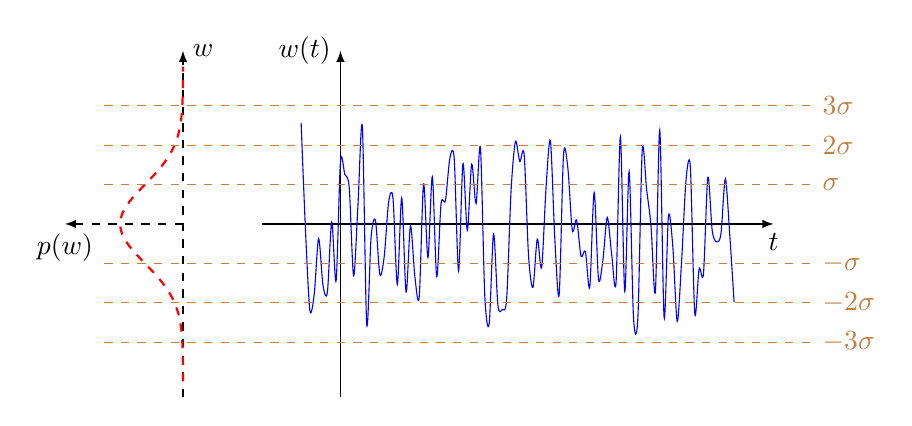
\begin{tikzpicture}
		\begin{scope}[shift={(0, 0)}]
			\draw[-latex] (-1,0) -- (5.5,0) node[below, align=center]{$t$};
			\draw[-latex] (0,-2.2) -- (0,2.2) node[left, align=right]{$w(t)$};
			\pgfmathsetseed{200};
			\draw[blue, smooth, domain=-0.5:5, samples=100] plot (\x,{1.3*rand});
		\end{scope}
		\begin{scope}[shift={(-2, 0)},rotate=90]
			\draw[-latex, dashed] (-2.2,0) -- (2.2,0) node[right, align=left]{$w$};
			\draw[-latex, dashed] (0,0) -- (0,1.5) node[below, align=center]{$p(w)$};
			\draw[red, thick, dashed, smooth, domain=-2:2, samples=50] plot (\x, {(1/(0.5*sqrt(2*pi)))*exp(-0.5*((\x)/0.5)^2)});
		\end{scope}
		\draw[brown, dashed] (-3, 1.5) -- ++(9,0) node[right,align=left]{$3 \sigma$};
		\draw[brown, dashed] (-3, 1.0) -- ++(9,0) node[right,align=left]{$2 \sigma$};
		\draw[brown, dashed] (-3, 0.5) -- ++(9,0) node[right,align=left]{$\sigma$};
		\draw[brown, dashed] (-3, -0.5) -- ++(9,0) node[right,align=left]{$-\sigma$};
		\draw[brown, dashed] (-3, -1.0) -- ++(9,0) node[right,align=left]{$-2 \sigma$};
		\draw[brown, dashed] (-3, -1.5) -- ++(9,0) node[right,align=left]{$-3 \sigma$};
	\end{tikzpicture}
	\caption[AWGN in the time domain]{\ac{AWGN} in the time domain}
\end{figure}

\begin{figure}[H]
	\centering
	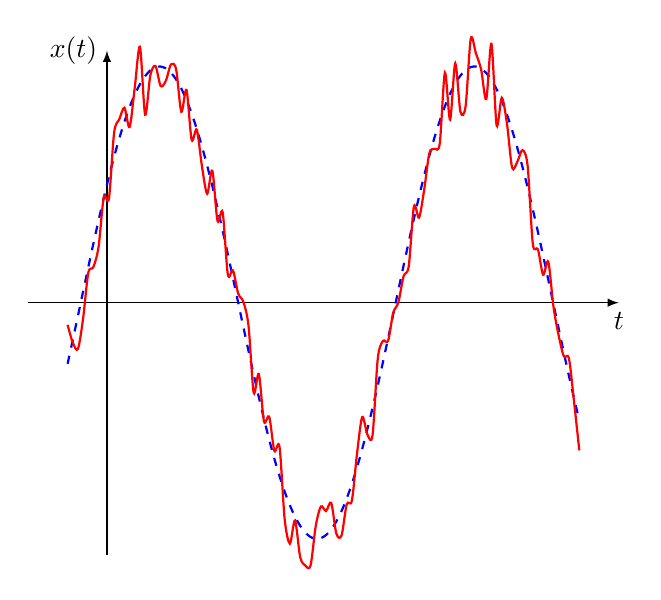
\begin{tikzpicture}
		\draw[-latex] (-1,0) -- (6.5,0) node[below, align=center]{$t$};
		\draw[-latex] (0,-3.2) -- (0,3.2) node[left, align=right]{$x(t)$};
		\draw[blue, thick, dashed, smooth, domain=-0.5:6, samples=100] plot (\x, {3*cos(360*\x/4-60)});
		\pgfmathsetseed{200};
		\draw[red, thick, smooth, domain=-0.5:6, samples=100] plot (\x, {3*cos(360*\x/4-60)+0.5*rand});
	\end{tikzpicture}
	\caption[Effect of AWGN on a signal (here monochromatic) in the time domain]{Effect of \ac{AWGN} on a signal (blue, here monochromatic) in the time domain. The resulting signal with the \ac{AWGN} is red.}
\end{figure}

\begin{figure}[H]
	\centering
	\begin{tikzpicture}
		\draw[-latex] (-3.2,0) -- (3.2,0) node[below, align=center]{$\Re$};
		\draw[-latex] (0,-3.2) -- (0,3.2) node[left, align=right]{$\Im$};
		\draw[blue, thick, dashed, -latex] (0:0) -- (60:2);
		\begin{scope}[shift={(60:2)}]
			\draw[brown, dashed] (0:0.4) arc(0:360:0.4);
			\draw[brown, dashed] (0:0.8) arc(0:360:0.8);
			\draw[brown, dashed] (0:1.2) arc(0:360:1.2);
			\draw[brown] (20:0.4) -- (20:2) node[right, align=left]{$\sigma$};
			\draw[brown] (45:0.8) -- (45:2.5) node[right, align=left]{$2 \sigma$};
			\draw[brown] (70:1.2) -- (70:3) node[right, align=left]{$3 \sigma$};
			\draw[brown, thick, -latex] (0:0) -- (130:0.5) node[anchor=east](W){};
		\end{scope}
		\draw[red, thick, -latex] (0,0) -- (W.east);
	\end{tikzpicture}
	\caption[Effect of AWGN on the phasor of a monochromatic signal (in the frequency domain)]{Effect of \ac{AWGN} (brown) on the phasor of a monochromatic signal (blue, in the frequency domain). The resulting signal with the \ac{AWGN} is red.}
\end{figure}

\subsection{Thermal Noise and Noise Floor}

The most important noise in electric circuits is \index{thermal noise} \textbf{thermal noise}.
\begin{itemize}
	\item Thermal noise is the corollary of oscillating atoms and molecules at the temperature $T$.
	\item The oscillation amplitude increases with increasing temperature. Consequently, the noise increases.
\end{itemize}

The noise \ac{PSD} $\mathrm{S}_{NN}$ is:
\begin{equation}
	\mathrm{S}_{NN}(\omega) = \frac{1}{2\pi} k_B T
\end{equation}
where $k_B = \SI{1.380649}{J/K}$ is the Boltzmann's constant. Or, for frequency instead of angular frequency:
\begin{equation}
	\mathrm{S}_{NN}(f) = k_B T
\end{equation}

\begin{itemize}
	\item When the thermal noise is band-limited, it has nearly a Gaussian or normal distribution. It is \ac{AWGN}.
	\item The noise has a finite power when it is band-limited.
\end{itemize}
The noise power of the band-limited thermal noise is
\begin{equation}
	\begin{split}
		P_N &= \int\limits_{\omega_1}^{\omega_2} \mathrm{S}_{NN} \; \mathrm{d} \omega \\
		 &= \frac{1}{2\pi} k_B T \underbrace{\left(\omega_2 - \omega_1\right)}_{= \Delta \omega} \\
		 &= k_B T \underbrace{\frac{\Delta \omega}{2\pi}}_{= \Delta f} \\
		 &= k_B T \Delta f
	\end{split}
\end{equation}
where $\Delta f$ is the \index{noise bandwidth} \textbf{noise bandwidth} in \si{Hz}.

\begin{excursus}{Noise in voltages and currents}
	The noise power is converted to a voltage or current, respectively, if it appears at an ohmic resistance.
	\begin{figure}[H]
		\centering
		\begin{circuitikz}
			\begin{scope}[shift={(0,0)}]
				\draw (0,0) to[R,l=$R$,o-o] ++(0,4);
				\node[align=center] at(0,-1) {Noisy\\ resistor};
			\end{scope}
			\begin{scope}[shift={(3,0)}]
				\draw (0,0) to[R,l=$R$,o-] ++(0,2) to[european voltage source,v={$U_{N,RMS}$},-o] ++(0,2);
				\node[align=center] at(0,-1) {Noise-free resistor\\ and noise\\ voltage source};
			\end{scope}
			\begin{scope}[shift={(6,0)}]
				\draw (3,0) to[short,o-] (0,0) to[european current source,i={$I_{N,RMS}$}] (0,4) to[short,-o] (3,4);
				\draw (2,0) to[R,l=$R$,*-*] (2,4);
				\node[align=center] at(1.5,-1) {Noise-free resistor\\ and noise current source};
			\end{scope}
		\end{circuitikz}
		\caption{Three equivalent circuits}
	\end{figure}

	Ohmic resistances are always noisy. They can be converted to an equivalent circuit:
	\begin{itemize}
		\item ideal noise-free resistor with noise voltage source, or
		\item ideal noise-free resistor with noise current source.
	\end{itemize}

	Let's consider the first equivalent circuit.
	\begin{figure}[H]
		\centering
		\begin{circuitikz}
				\draw (0,0) to[R,l=$R$,o-] ++(0,2) to[european voltage source,v={$U_{N,RMS}$},-o] ++(0,2);
				\draw (0,0) to[short] (2,0) to[R,l=$R$] (2,4) to[short] (0,4);
		\end{circuitikz}
		\caption{The maximum power is transferred to a load of the same impedance as the inner resistance.}
	\end{figure}
	A load is connected to the noise source. To obtain a maximum power transfer, the load's impedance must equal the inner resistance of the source. The power emitted by the voltage source is:
	\begin{equation}
		P_N = \frac{U_{N,RMS}^2}{4 R}
	\end{equation}
	The noise voltage is:
	\begin{equation}
		U_{N,RMS} = \sqrt{4 k_B T \Delta f R}
	\end{equation}
	
	Analogue to the voltage, the noise current is:
	\begin{equation}
		I_{N,RMS} = \sqrt{\frac{4 k_B T \Delta f}{R}}
	\end{equation}
\end{excursus}

\paragraph{Noise Floor.}

The noise \ac{PSD} is small compared to the signals carrying information. Therefore, the logarithmic scale is used.

The noise \ac{PSD} level is
\begin{equation}
	L_{S,N} = \SI{10}{dBm/Hz} \log_{10} \left(\frac{k_B T}{\SI{1}{mW/Hz}}\right)
\end{equation}

\begin{itemize}
	\item The noise power is equally distributed over the frequency.
	\item Therefore, the \ac{PSD} is flat in the frequency domain, which is called \index{noise floor} \textbf{noise floor}.
\end{itemize}

\begin{fact}
	The noise \ac{PSD} or noise floor at room temperature (\SI{25}{\degreeCelsius} or $T = \SI{298.15}{K}$) is $L_{S,N} = \SI{-173.8}{dBm/Hz} \approx \SI{-174}{dBm/Hz}$.
\end{fact}

Band-limiting the noise, yields the noise power. The noise power is:
\begin{equation}
	\begin{split}
		L_{P,N} &= \SI{10}{dBm} \log_{10} \left(\frac{k_B T \Delta f}{\SI{1}{mW}}\right) \\
		 &= L_{S,N} + \SI{10}{dBHz} \log_{10} \left(\frac{\Delta f}{\SI{1}{Hz}}\right)
	\end{split}
\end{equation}

Here, the advantage of the logarithmic scale comes into play. For example, a \ac{LTE} signal with a bandwidth of $\Delta f_{LTE} = \SI{20}{MHz}$ has a noise power of $\SI{-174}{dBm/Hz} + \SI{73}{dBHz} = \SI{-101}{dBm}$.

\subsection{Signal-to-Noise Ratio and Noise Figure}

\paragraph {The Signal-to-Noise Ratio.}

Following scenario:
\begin{itemize}
	\item There is a signal at a frequency $\omega_0$ with a \ac{PSD} of $L_{S,X1}$ (for example indefinitely small peak $L_{S,X1} = \SI{-10}{dBm/Hz}$).
	\item The noise floor is the thermal noise $L_{S,N1}$ (for example $L_{S,N1} = \SI{-174}{dBm/Hz}$).
	\item The bandwidth considered is $\Delta f$ (for example $\Delta f = \SI{20}{MHz}$).
\end{itemize}

\begin{figure}[H]
	\centering
	\begin{tikzpicture}
		\draw[-latex] (-0.5,0) -- (5,0) node[below, align=center]{$f$\\ in $\si{Hz}$};
		\draw[-latex] (0,-10) -- (0,1) node[left, align=right]{$S(f)$\\ in $\si{dBm/Hz}$};
		
		\draw (2,0) -- ++(0,-0.1) node[below right, align=left]{$\omega_0$};
		
		\draw (0,-8.7) -- ++(-0.1,0) node[left, align=right]{$-174$};
		\draw (0,-0.5) -- ++(-0.1,0) node[left, align=right]{$-10$};
		
		\draw[red, thick] (0,-8.7) -- ++(5,0) node[above left, align=right]{Noise floor};
		\draw[blue, thick, -o] (2,-8.7) -- (2,-0.5) node[below right, align=left]{Signal};
	\end{tikzpicture}
	\caption[A signal including the AWGN]{A signal including the \ac{AWGN}}
\end{figure}

The noise power (level) is:
\begin{equation}
	\begin{split}
		P_{N1} &= \SI{1}{mW/Hz} 10^{\frac{L_{S,N1}}{\SI{10}{dBm/Hz}}} \cdot \Delta f \\
		L_{P,N1} &= L_{S,N1} + \SI{10}{dBHz} \log_{10} \left(\frac{\Delta f}{\SI{1}{Hz}}\right)
	\end{split}
\end{equation}
In this example, $L_{P,N1} = \SI{-101}{dBm}$.

The signal power is obtained by integrating the signal \ac{PSD} over the bandwidth:
\begin{equation}
	P_{X1} = \int\limits_{\Delta f} S_{XX}(\omega) \; \mathrm{d} \omega
\end{equation}

The signal \ac{PSD} in this example is:
\begin{equation*}
	S_{XX}(\omega) = \delta(\omega \pm \omega_0) \SI{1}{mW/Hz} 10^{\frac{L_{S,X1}}{\SI{10}{dBm/Hz}}}
\end{equation*}
In this example $P_{X1} \equiv L_{P,X1} = \SI{-10}{dBm}$.

\textit{Note:} the signal is just a indefinite small peak (Dirac delta function). All of its power is concentrated in its peak, so that the bandwidth does not matter. This signal does not exist in practise, but this is just an exemplary consideration.

\begin{definition}{Signal-to-noise ratio}
	The \index{signal-to-noise ratio} \textbf{\ac{SNR}} is the ratio between the signal power $P_{X}$ and the noise power $P_{N}$:
	\begin{equation}
		\mathrm{SNR} = \frac{P_{X}}{P_{N}}
	\end{equation}%
	\nomenclature[Ss]{$\mathrm{SNR}$}{Signal-to-noise ratio}
	
	Or in logarithmic scale
	\begin{equation}
		L_{\mathrm{SNR}} = \SI{10}{dB} \log_{10} \left(\frac{P_{X}}{P_{N}}\right) = L_{P,X} - L_{P,N}
	\end{equation}
\end{definition}

In this example, the \ac{SNR} is $L_{\mathrm{SNR},1} = \SI{91}{dB}$.

Often, the noise floor is defined to be \SI{91}{dBc}, which means that the noise is \SI{91}{dB} below the \index{carrier} \emph{carrier} -- the signal carrying the information.

\paragraph{\ac{SNR} Degradation.}

The signal including the \ac{AWGN} is applied to a system with a \index{gain} \textbf{gain} $G$.

Gain in logarithmic scale:
\begin{equation}
	L_G = \SI{10}{dB} \log_{10} \left(G\right)
\end{equation}

\begin{itemize}
	\item Positive log. gain $L_G > 0$ ($G > 1$): amplifier
	\item Negative log. gain $L_G < 0$ ($0 \leq G < 1$): attenuator
\end{itemize}

\begin{figure}[H]
	\centering
	\begin{tikzpicture}
		\node[draw, block](Sys){System\\ (gain $G$,\\ noise factor $F$)};
		
		\draw[-o] (Sys.west) -- ++(-2,0) node[left, align=right]{Input\\ $P_{X1} + P_{N1}$};
		\draw[-o] (Sys.east) -- ++(2,0) node[right, align=left]{Output\\ $P_{X2} + P_{N2}$};
	\end{tikzpicture}
	\caption[A system with gain degrading the SNR]{A system with gain degrading the \ac{SNR}}
\end{figure}

The system
\begin{itemize}
	\item amplifies or attenuates \underline{both} the signal \underline{and} the noise, and
	\item adds intrinsic \ac{AWGN}.
\end{itemize}

The intrinsic \ac{AWGN} is thermal noise generated inside the system. This additional noise contribution shows up as an additional increase of the noise floor by a factor $F$ -- the \index{noise factor} \textbf{noise factor}. Or in logarithmic scale:
\begin{equation}
	L_F = \SI{10}{dB} \log_{10} \left(F\right)
\end{equation}

\begin{itemize}
	\item Amplification or attenuation of the signal:
	\begin{itemize}
		\item Linear scale: $P_{X2} = G P_{X1}$
		\item Logarithmic scale: $L_{P,X2} = L_{P,X1} + L_G$
	\end{itemize}
	\item Amplification or attenuation of the noise \underline{plus} intrinsic noise contribution:
	\begin{itemize}
		\item Linear scale: $P_{N2} = G F P_{N1}$
		\item Logarithmic scale: $L_{P,N2} = L_{P,N1} + L_G + L_F$
	\end{itemize}
\end{itemize}

The additional contribution of \ac{AWGN}, degrades the \ac{SNR} by $L_F$.

\begin{definition}{Noise figure and noise factor}
	The \index{noise factor} \textbf{noise factor} $F$ is the ratio of input \ac{SNR} $\mathrm{SNR}_i$ to output \ac{SNR} $\mathrm{SNR}_o$.
	\begin{equation}
		F = \frac{\mathrm{SNR}_i}{\mathrm{SNR}_o}
	\end{equation}
	
	In logarithmic scale, the ratio is expressed by the \index{noise figure} \textbf{noise figure} $L_F$.
	\begin{equation}
		L_F = \SI{10}{dB} \log_{10} \left(F\right) = L_{\mathrm{SNR},i} - L_{\mathrm{SNR},o}
	\end{equation}
\end{definition}

\begin{figure}[H]
	\centering
	\begin{tikzpicture}
		\begin{scope}[shift={(0,0)}]
			\draw[-latex] (-0.5,0) -- (5,0) node[below, align=center]{$f$\\ in $\si{Hz}$};
			\draw[-latex] (0,-10) -- (0,1.5) node[left, align=right]{$S(f)$\\ in $\si{dBm/Hz}$};
			
			\draw (2,0) -- ++(0,-0.1) node[below right, align=left]{$\omega_0$};
			
			\draw (0,-8.7) -- ++(-0.1,0) node[left, align=right]{$-174$};
			\draw (0,-0.5) -- ++(-0.1,0) node[left, align=right]{$-10$};
			
			\draw[red, thick] (0,-8.7) -- ++(5,0) node[above left, align=right](N1){Noise floor};
			\draw[blue, thick, -o] (2,-8.7) -- (2,-0.5) node[below right, align=left](X1){Signal};
		\end{scope}
		\begin{scope}[shift={(8,0)}]
			\draw[-latex] (-0.5,0) -- (5,0) node[below, align=center]{$f$\\ in $\si{Hz}$};
			\draw[-latex] (0,-10) -- (0,1.5) node[left, align=right]{$S(f)$\\ in $\si{dBm/Hz}$};
			
			\draw (2,0) -- ++(0,-0.1) node[below right, align=left]{$\omega_0$};
			
			\draw (0,-8.7) -- ++(-0.1,0) node[left, align=right]{$-174$};
			\draw (0,-7.7) -- ++(-0.1,0) node[left, align=right]{$-154$};
			\draw (0,-7.2) -- ++(-0.1,0) node[left, align=right]{$-144$};
			\draw (0,-0.5) -- ++(-0.1,0) node[left, align=right]{$-10$};
			\draw (0,0.5) -- ++(-0.1,0) node[left, align=right]{$+10$};
			
			\draw[red, dashed] (0,-7.7) -- ++(5,0) node[below left, align=right](Ng){Noise (gain only)};
			\draw[red, thick] (0,-7.2) -- ++(5,0) node[above left, align=right](N2){Noise floor};
			\draw[blue, thick, -o] (2,-7.2) -- (2,0.5) node[above right, align=left](X2){Signal};
		\end{scope}
		\begin{scope}[shift={(6,0)}]
			\draw (-0.5,-8.7) -- (0.5,-8.7);
			\draw[<->] (0,-8.7) -- (0,-7.7) node[midway, left, align=right]{$L_G$};
			\draw (-0.5,-7.7) -- (0.5,-7.7);
			\draw[<->] (0,-7.7) -- (0,-7.2) node[midway, left, align=right]{$L_F$};
			\draw (-0.5,-7.2) -- (0.5,-7.2);
			\draw (-0.5,-0.5) -- (0.5,-0.5);
			\draw[<->] (0,-0.5) -- (0,0.5) node[midway, left, align=right]{$L_G$};
			\draw (-0.5,0.5) -- (0.5,0.5);
		\end{scope}
	\end{tikzpicture}
	\caption[Degradation of the SNR]{Degradation of the \ac{SNR}}
\end{figure}

In our example:
\begin{itemize}
	\item System properties:
	\begin{itemize}
		\item Gain $L_G = \SI{20}{dB}$
		\item Noise figure $L_F = \SI{10}{dB}$
	\end{itemize}
	\item Output signal power $L_{X2} = \SI{+10}{dBm}$
	\item Output noise power $L_{X2} = \SI{-71}{dBm}$ ($\SI{-144}{dBm/Hz}$ at $\SI{20}{MHz}$)
	\item \ac{SNR} $L_{\mathrm{SNR},o} = \SI{81}{dB}$
\end{itemize}

\paragraph{Cascading Systems.}

In a cascade of systems, the gain $G$ and noise factor $F$ must be applied several times.

\begin{definition}{Friis formula}
	The total noise factor of a chain of $n$ devices can be calculated by the \index{Friis formula} \textbf{Friis formula}.
	\begin{equation}
		F_{\text{total}} = F_1 + \frac{F_2 - 1}{G_1} + \frac{F_3 - 1}{G_1 G_2} + \frac{F_4 - 1}{G_1 G_2 G_3} + \dots + \frac{F_n - 1}{G_1 G_2 \dots G_{n-1}}
	\end{equation}
	$F$ and $G$ are in linear scale (not logarithmic scale).
	
	\begin{figure}[H]
		\centering
		\begin{adjustbox}{scale=0.8}
			\begin{tikzpicture}
				\node[draw, block](S1){System\\ ($G_1$, $F_1$)};
				\node[draw, block,right=of S1](S2){System\\ ($G_2$, $F_2$)};
				\node[block,right=of S2](Sd){$\dots$};
				\node[draw, block,right=of Sd](Sn){System\\ ($G_n$, $F_n$)};
				
				\draw[latex-] (S1.west) -- ++(-1,0) node[left, align=right]{Source};
				\draw[-latex] (S1.east) -- (S2.west);
				\draw[-latex] (S2.east) -- (Sd.west);
				\draw[-latex] (Sd.east) -- (Sn.west);
				\draw[-latex] (Sn.east) -- ++(1,0) node[right, align=left]{Output};
				
				\draw[decorate, decoration={brace, amplitude=3mm, mirror}] (S1.south west) -- (Sn.south east) node[midway, anchor=north, yshift=-4mm]{$G_{\text{total}}$, $F_{\text{total}}$};
			\end{tikzpicture}
		\end{adjustbox}
	\end{figure}
\end{definition}

\textit{Remark:} The total chain gain is:
\begin{equation}
	G_{\text{total}} = G_1 G_2 \dots G_n = \prod_{i = 1}^{n} G_i
\end{equation}

\phantomsection
\addcontentsline{toc}{section}{References}
\printbibliography[heading=subbibliography]
\end{refsection}

